% \chapter{Accelerating Simulations with AI}
% \label{sec:04_ml4sim}

\ifdefined\HCode
    \chapter{Introduction and the JetNet Dataset}
\else
    \chapter{Introduction and the \jetnet Dataset}
\fi
\label{sec:04_intro}

\begin{center}
    \parbox{.8\linewidth}{%
        \centering
        \noindent
        \textit{What I cannot create, I do not understand.}
        - Richard Feynman
    }
\end{center}

Simulations are critical components of the scientific process in high-energy physics.
They are employed from the beginning of the experimental design, to evaluate the expected performance of a detector, all the way up to the data analysis, to determine our sensitivity to a given signal process.

For the CMS experiment, the simulation pipeline broadly involves:
\begin{enumerate}
    \item Event generation: simulating the hard collision process, parton showering, hadronization, and underlying event interactions (see Chapter~\ref{sec:01_sm_qcd}), outputting generator-level or ``gen-level'' particles.
    \item Detector simulation: simulating the response of the detector to the particles produced in the collision and outputting the raw detector signals, or ``hits'' in the detector, most commonly with the \GEANTfour software~\cite{Agostinelli:2002hh}.
    \item Reconstruction: converting the raw detector signals into tracks and ECAL/HCAL clusters, which can then be reconstructed further into physical ``objects'' like jets, leptons, and missing transverse energy (see Chapter~\ref{sec:02_cms_reconstruction}).
\end{enumerate}

The first two steps are inherently stochastic processes due to the randomness of quantum mechanical decays and interactions between particles and materials.
This means that the complete analytic form for the probability densities of collision and detector outputs is intractable.
Instead, traditionally, the event generation relies on Monte Carlo (MC) methods to sample from probability distributions of decays and interactions, while the detector simulation propagates the resulting particles through the detector and magnetic field, simulating the random interactions and energy deposits at each step.

These methods have proven extremely effective at modeling collisions and the detector response for decades in HEP, but are computationally expensive: the full simulation of a single collision in CMS takes $\mathcal O(10\unit{s})$~\cite{Pedro:2018jqu}.
To maximize the physics potential of the upcoming era of high luminosity, the CMS experiment will need to reconstruct 300 billion real collision events, and
simulate and reconstruct 2--3$\times$ more, a monumental task to which current methods cannot scale.
Indeed, we are expected to fall 3--10$\times$ short of the necessary CPU resources to do this in HL-LHC~\cite{CMS:2815292}.

There are two important avenues of R\&D which must be explored to address this.
First, performing simulation and reconstruction on GPUs: even porting a conservative fraction can improve computing capacity by 20-26\%.
% , but it is unclear whether the sequential nature of simulation can translate well.
Second, wide adoption of a fast simulation and reconstruction alternative (FastSim): 50\% of CMS analyses switching to this would mean a 10$\times$ speed-up in simulations, which are in total expected to require 40\% of CPU resources~\cite{CMS:2815292}.
However, they each carry risks: of simulations not translating well to GPUs due to their sequential nature, and of inadequate FastSim performance leading to insufficient adoption by analyzers.
% ~\cite{CMS:2815292}.

ML advancements in generative modeling can simultaneously improve the quality of fast simulations and naturally enable GPU-acceleration, addressing both risks.
In this Part, we introduce such advancements using novel physics-informed deep learning (DL) generative models, and efficient and sensitive techniques for their validation.

We first introduce below the problem of simulating high energy jets and introduce the \jetnet benchmark dataset used for all studies in the chapter.
As highlighted in Chapter~\ref{sec:03_ml}, a key contribution of this work is use of particle-cloud representations of jets, which we argued are more natural for HEP data than the more common (at the time) image- and vector-based algorithms.
% We also discuss representations of jets, as a key result of this work is the success, for the first time, of point-cloud, or ``particle-cloud'', representations for simulating HEP data, as opposed to the more common (at the time) image- and vector-based algorithms.

To that end, we introduce two novel and highly performant ML-based approaches designed to leverage point clouds in HEP, using (1) message-passing graph neural networks (GNNs) (Chapter~\ref{sec:04_mpgan}) and (2) attention-based transformer networks (Chapter~\ref{sec:04_gapt}).
We will then discuss the critical problem of validating such ML-based fast simulation techniques and propose two new, sensitive methods to do so (Section~\ref{sec:04_evaluating}).
We will finally conclude with the outlook for these techniques in Chapter~\ref{sec:04_outlook}, discussing as well how this work has sparked a new, vibrant subfield of ML research in HEP.
% and ultimately their potential to revolutionize the HEP computing paradigm.

% \chapter{Jets and the \texorpdfstring{\jetnet}{JetNet} dataset}
% \label{sec:04_jetnet}

\section{Simulating jets}
\label{sec:04_jetnet_jets}

We test the performance of our generative models on the simulation of high energy jets, from parton-level inputs through parton showering and hadronization up to emulating the detector response.
% Jets and their current methods of simulation are reviewed in Section~\ref{sec:04_jetnet_jets}.
% We then introduce the \jetnet dataset in Section~\ref{sec:04_jetnet_dataset}, which will be used as a test bench for all our models, and discuss the various representations of jets in the context of ML in Section~\ref{sec:04_jetnet_representations}.
As discussed in Chapter~\ref{sec:01_sm_qcd}, high-energy proton-proton collisions at the LHC produce elementary particles like quarks and gluons, which cannot be isolated due to the QCD property of color confinement.
These particles continuously radiate or into sets of particles, a process referred to as parton showering.
Eventually, they cool to an energy at which they undergo the process of hadronization, where the fundamental particles combine to form color-neutral hadrons, such as pions and protons.
The final set of collimated hadrons produced after such a process is referred to as a jet.

The task of simulating a single jet can be algorithmically defined as inputting an initial particle, which produces the jet, and outputting the final set of particles a.k.a. the jet constituents.
Typically in HEP the parton shower and hadronization are steps that are simulated sequentially using MC event generators such as \PYTHIA~\cite{pythia} or \HERWIG~\cite{herwig}.
Simulating either process exactly is not possible because of the nonperturbative nature of QCD at low energies, and instead these event generators fit simplified physics-inspired stochastic models, such as the Lund string model for hadronization~\cite{Andersson:1983ia}, to existing data using MC methods.
% These models are then used to generate more data for use in analyses.
The present work can be seen as an extension of this idea, using a simpler, ML-based model, also fitted to data, for generating the jet in one shot.
Effectively, we are trading the interpretability of MC methods for the speed of GPU-accelerated ML generators.


\ifdefined\HCode
    \section{JetNet}
\else
    \section{\texorpdfstring{\jetnet}{JetNet}}
\fi

\label{sec:04_jetnet_dataset}

\begin{figure}[t!]
    \centering
    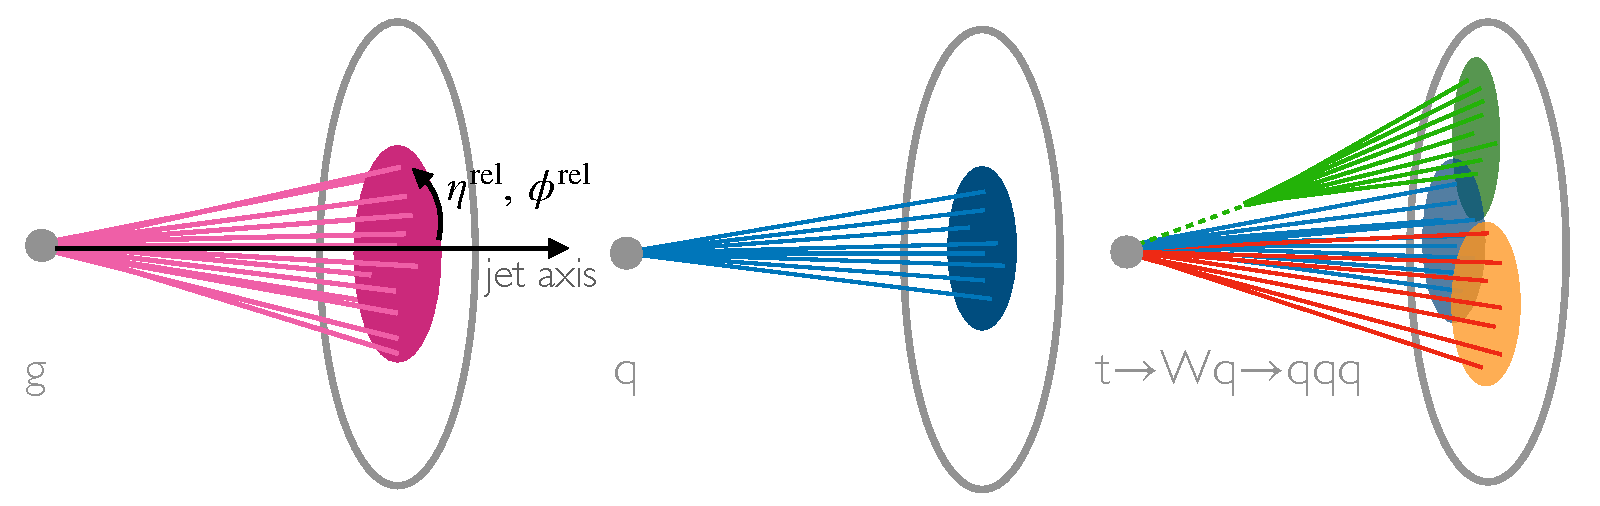
\includegraphics[width=0.74\textwidth]{figures/04-ML4Sim/jets/jetcartoon.pdf}
    \caption[The three jet classes we simulate.]{
    The three jet classes we simulate.
    Gluon (g) and light quark (q) jets have simple topologies, with q jets generally containing fewer particles.
    Top quark (t) jets have a complex three-pronged structure.
    Shown also are the relative angular coordinates $\etarel$ and $\phirel$, measured from the jet axis.}
    \label{fig:04_jetcartoon}
\end{figure}

We introduce the \jetnet dataset as a benchmark dataset for studies of fast simulation techniques in high-energy physics.
It is derived from Ref.~\cite{hls4mldata_150p},\footnote{This dataset was released under the CC-BY 4.0 license.} and comprises simulated particle jets with transverse momenta $p_{\mathrm{T}}^{\mathrm{jet}}\approx 1\TeV$, originating from gluons, light quarks, top quarks, and \PW and \PZ bosons produced in $13\TeV$ proton-proton collisions through a simplified detector (Figure~\ref{fig:04_jetcartoon}).

As disucssed in Chapter~\ref{sec:03_ml}, each jets is represented as a point cloud, or \textit{particle cloud}, of particles, with each particle represented as a node in the cloud with the three kinematic $(\ptrel, \etarel, \phirel)$ features.
$\pt, \eta, \phi$ are the transverse momentum, pseudorapidity, and azimuthal angle, respectively, commonly used in collider physics and defined in Chapter~\ref{sec:02_cms}.
\ptrel is the transverse momentum of the particle relative to the jet \pt, and $\etarel$ and $\phirel$ are the particle's angular coordinates relative to the jet axis.

Details of the simulations are as follows.
The parton-level events are first produced at leading-order using \MGvATNLO2.3.1~\cite{Alwall:2011uj} with the NNPDF\,2.3LO1 parton distribution functions~\cite{Ball:2012cx}.
To focus on a relatively narrow kinematic range, the transverse momenta of the partons and undecayed gauge bosons are generated in a window with energy spread given by $\Delta \pt / \pt = 0.01$, centered at $1\TeV$.
These parton-level events are then decayed and showered in \PYTHIA8.212~\cite{pythia} with the Monash 2013 tune~\cite{Skands:2014pea}, including the contribution from the underlying event.
For each original particle type, 200,000 events are generated.
Jets are clustered using the anti-$\kt$ algorithm~\cite{Cacciari:2008gp}, with a distance parameter of $R = 0.8$ using the \textsc{FastJet}~3.1.3 and \textsc{FastJet~contrib}~1.027 packages~\cite{fastjet:1,fastjet:2}.
Even though the parton-level $\pt$ distribution is narrow, the jet $\pt$ spectrum is significantly broadened by kinematic recoil from the parton shower and energy migration in and out of the jet cone.
We apply a restriction on the measured jet $\pt$ to remove extreme events outside of a window of $0.8\TeV < \pt < 1.6\TeV$ for the $\pt = 1\TeV$ bin.
This generation is a significantly simplified version of the official simulation and reconstruction steps used for real detectors at the LHC, to remain experiment-independent as well as allow public access to the dataset.


\subsubsection{Acknowledgements}

This chapter is, in part, a reprint of the materials as they appear in
NeurIPS, 2021, R. Kansal; J. Duarte; H. Su; B. Orzari; T. Tomei; M. Pierini; M. Touranakou; J.-R. Vlimant; and D. Gunopulos. Particle Cloud Generation with Message Passing Generative Adversarial Networks.
The dissertation author was the primary investigator and author of this paper.
